\documentclass[9pt]{IEEEtran}

\usepackage[english]{babel}
\usepackage{graphicx}
\usepackage{epstopdf}
\usepackage{fancyhdr}
\usepackage{amsmath}
\usepackage{amsthm}
\usepackage{amssymb}
\usepackage{url}
\usepackage{array}
\usepackage{textcomp}
\usepackage{listings}
\usepackage{hyperref}
\usepackage{xcolor}
\usepackage{colortbl}
\usepackage{float}
\usepackage{gensymb}
\usepackage{longtable}
\usepackage{supertabular}
\usepackage{multicol}

\usepackage[utf8x]{inputenc}

\usepackage[T1]{fontenc}
\usepackage{lmodern}{}
\input{glyphtounicode}
\pdfgentounicode=1

\graphicspath{{./figures/}}
\DeclareGraphicsExtensions{.pdf,.png,.jpg,.eps}

% correct bad hyphenation here
\hyphenation{op-tical net-works semi-conduc-tor trig-gs}

% ============================================================================================

\title{\vspace{0ex}
Mean-Shift tracking}

\author{Marko Medved\vspace{-4.0ex}}

% ============================================================================================

\begin{document}

\maketitle

\section{Introduction}

\section{Experiments}
\subsection{Kalman filtering}
In this section we derived the input matrices (see Appendix) for the Random walk (RW), 
Nearly constant velocity (NCV) and Nearly constant acceleration (NCA) motion 
models. We tested all these models on three different trajectories. \\

Firstly on Figures~\ref{fig:kf1},~\ref{fig:kf2} and~\ref{fig:kf3} we can 
see the trajectories and their filtered counterparts in dependence to different 
motion models as well as constants for dynamics noise(q) and measurement 
covariance(r). On all three plots, for all three motion models, we can see that when setting a large q and small 
r the Filtered measurements follow the measurements nicely, which is expected 
since we assign more uncertainty to the dynamics, so our tracker mostly uses the 
measurements for prediction. \\

On the other hand, when setting a high r and low q 
we are relying more on the motion model. We can see that because the tracker relies 
mostly on the motion models, the random walk cannot follow the path fast enough. As 
for the NCV and NCA models, we can see that the paths start to differ a lot from 
the measurements, especially in the second plot. This is not necesarilly a bad thing, since 
in situations where our measurements are poor, the tracker will perform better, since it 
will rely more on the motion model. \\

The optimal parameters are dependent on the choice of motion model and specific application.
For RW we should rely more on the measurements so maybe $q=5$ and $r=1$ would be 
acceptable. For the NCV and NCA models we can rely more on the motion model 
so we can pick a larger r. 

\begin{figure}[h]
    \centering
    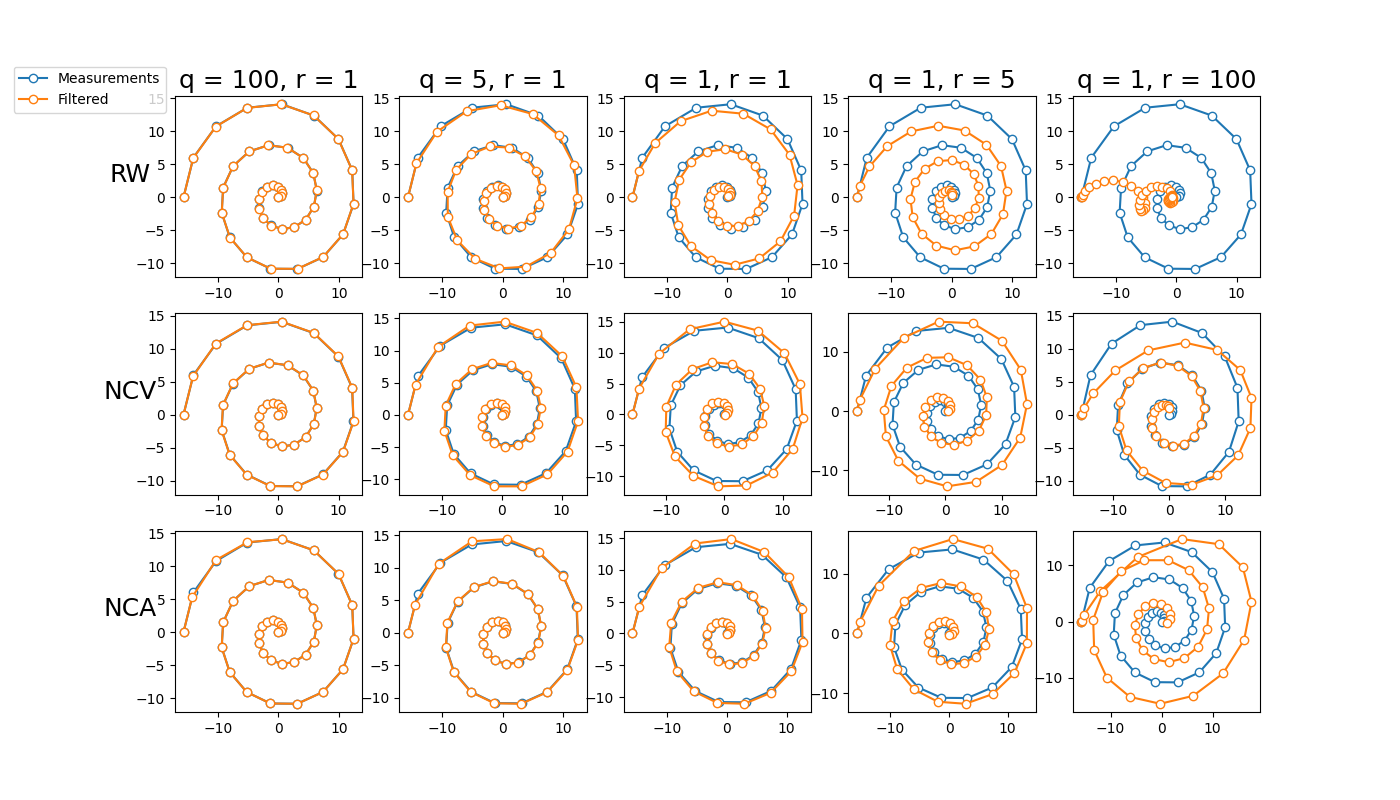
\includegraphics[width=0.99\columnwidth]{figures/0.png}
    \caption{Kalman filtering method on the spiral curve}
    \label{fig:kf1}
\end{figure}

\begin{figure}[h]
  \centering
  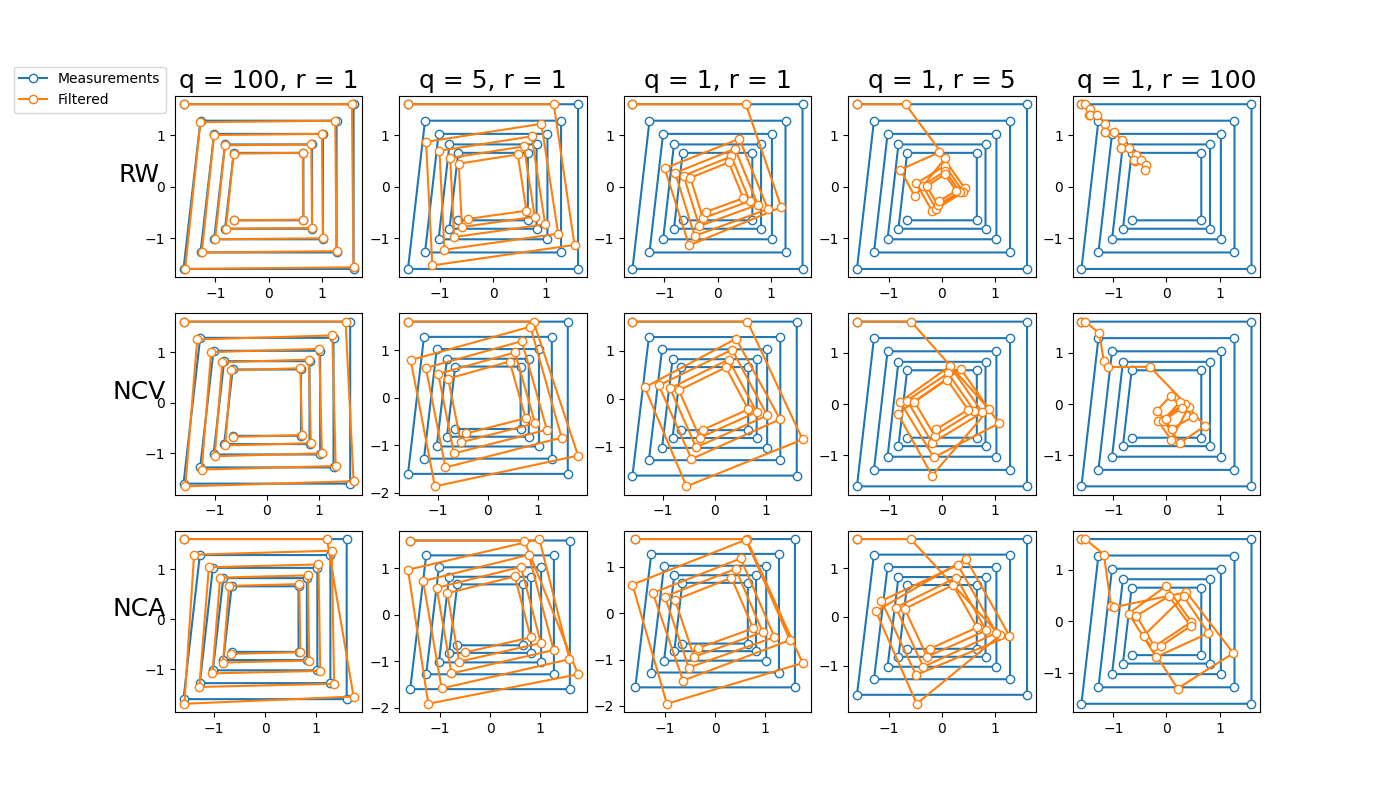
\includegraphics[width=0.99\columnwidth]{figures/1.png}
  \caption{Kalman filtering method on the square spiral curve}
  \label{fig:kf2}
\end{figure}

\begin{figure}[h]
  \centering
  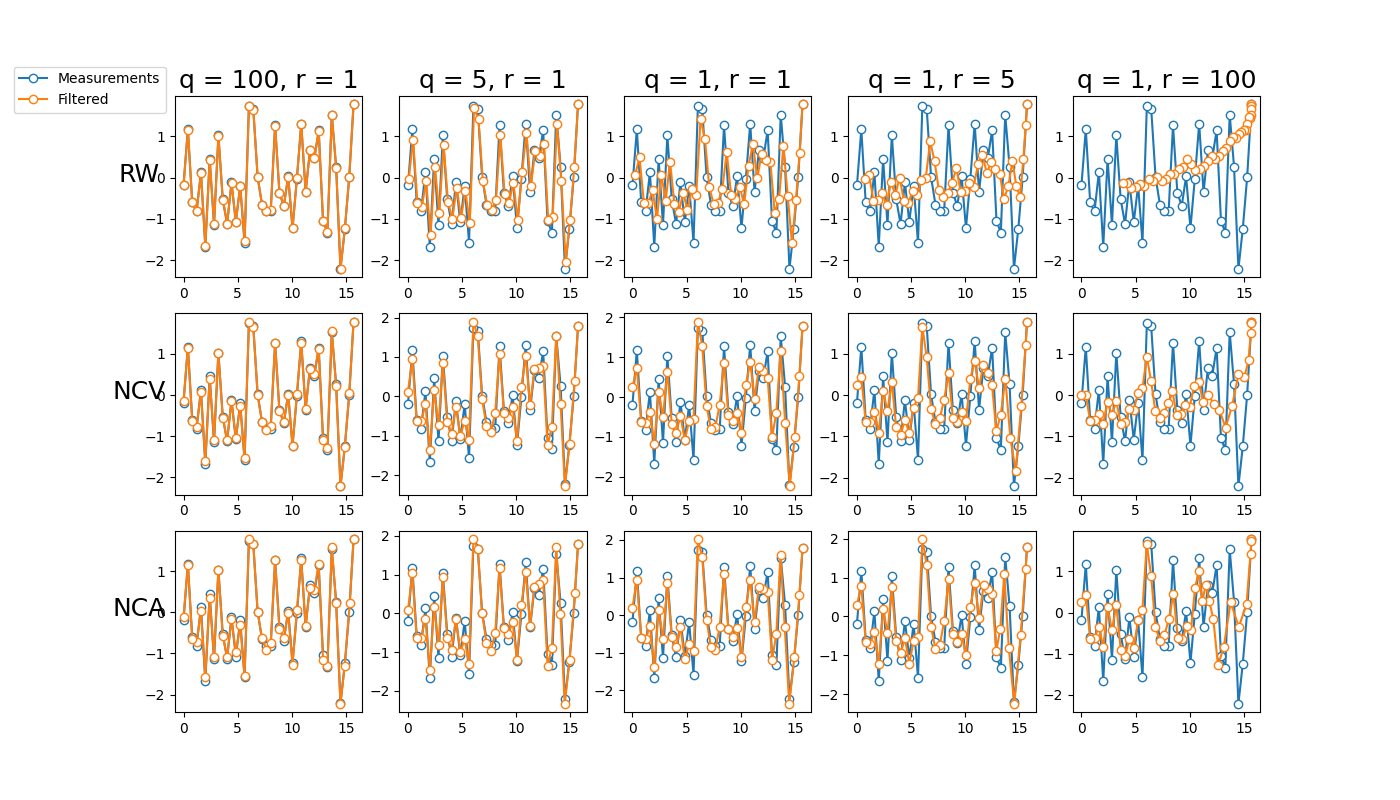
\includegraphics[width=0.99\columnwidth]{figures/2.png}
  \caption{Kalman filtering method on random gaussian noise}
  \label{fig:kf3}
\end{figure}

\subsection{Results of the basic particle filter tracker implementation}
Here we implemented the particle filter tracker using the NCV motion model 
and color histograms for the visual model. We can observe the results for the 
entire VOT 2014 dataset in 
Table~\ref{tab:pf_tracker_results}. Note that we used an update speed 
$\alpha = 0.00001$, kernel size $\sigma = 1$, 16 bins in the histogram, the
 dynamic noise constant was $80\%$ of the size of the smaller dimension of the 
 patch and the number of particles was set to 100.

\begin{table}[h]
  \centering
  \begin{tabular}{l|c}

  \textbf{Metric} & \textbf{Value} \\
  \hline 
  Average Overlap & 0.52 \\
  Total Failures & 32 \\
  Average Speed (FPS) & 86.76 \\

  \end{tabular}
  \vspace{3pt}
  \caption{Basic particle tracker performance}
  \label{tab:pf_tracker_results}
  \end{table}

\subsection{Testing using different motion models}
We tested the tracker using all of the three aforementioned motion models. 
For each of the models we tested various different dynamic noise constants(q). 
We can see the number of failures as well as average overlap when using for 
different parameters in Figure~\ref{fig:motion_models}. 

\begin{figure}[h]
  \centering
  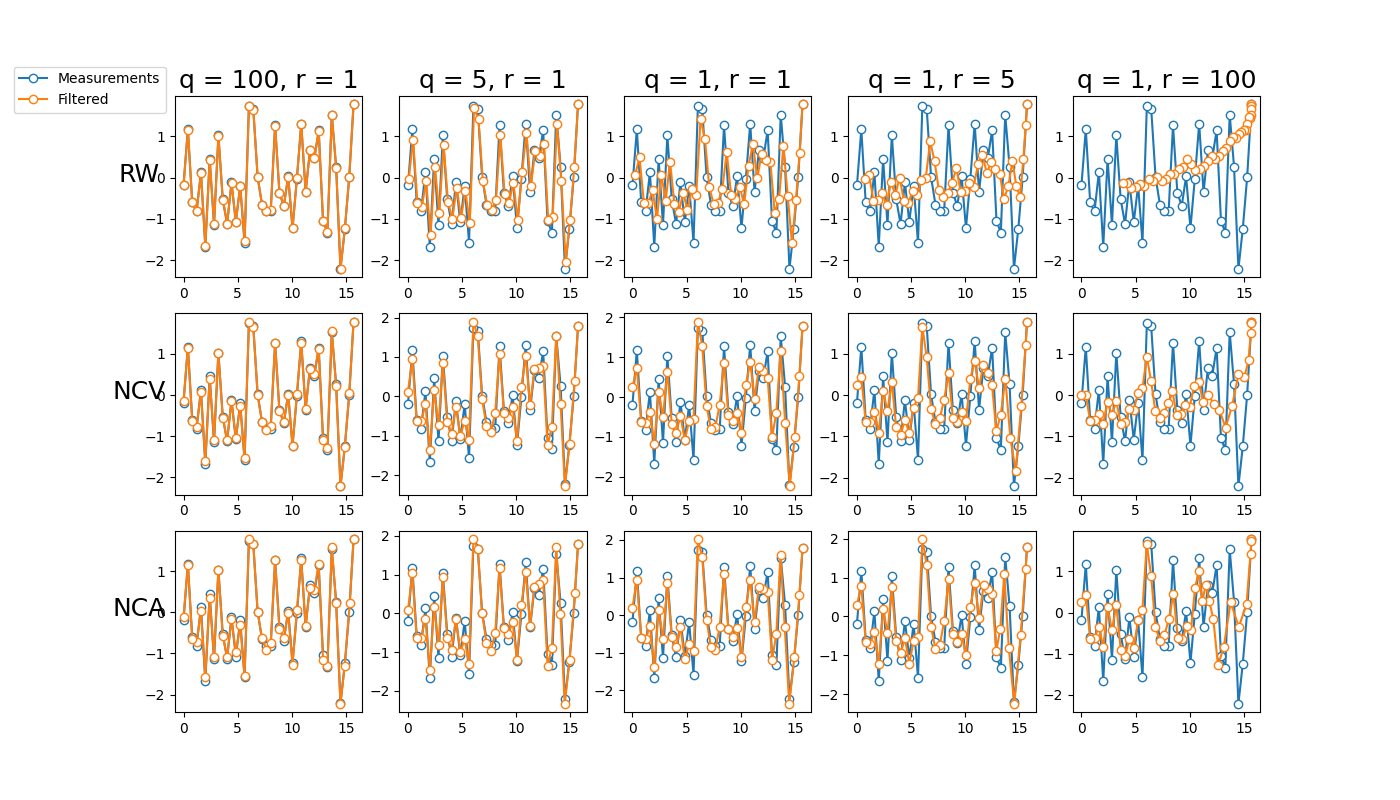
\includegraphics[width=0.99\columnwidth]{figures/2.png}
  \caption{}
  \label{fig:motion_models}
\end{figure}

\subsection{Testing the influence of number of particles}



\clearpage
\newpage
\section{Appendix}
Here we present the matrices derived for the motion models
\subsection{Random walk}
\[
\mathbf{X} = \begin{bmatrix} x \\ y \end{bmatrix}, \quad
\mathbf{F} = \begin{bmatrix} 0 & 0 \\ 0 & 0 \end{bmatrix}, \quad
\boldsymbol{\phi} = \begin{bmatrix} 1 & 0 \\ 0 & 1 \end{bmatrix}, \quad
\mathbf{L} = \begin{bmatrix} 1 & 0 \\ 0 & 1 \end{bmatrix}, \quad
\mathbf{Q} = \begin{bmatrix} \Delta t\,q & 0 \\ 0 & \Delta t\,q \end{bmatrix}, \quad
\mathbf{H} = \begin{bmatrix} 1 & 0 \\ 0 & 1 \end{bmatrix}
\]


\subsection{Nearly constant velocity}
\[
\mathbf{X} = 
\begin{bmatrix}
x \\
y \\
\dot{x} \\
\dot{y}
\end{bmatrix}, \quad
\mathbf{F} = 
\begin{bmatrix}
0 & 0 & 1 & 0 \\
0 & 0 & 0 & 1 \\
0 & 0 & 0 & 0 \\
0 & 0 & 0 & 0
\end{bmatrix}, \quad
\boldsymbol{\Phi} = 
\begin{bmatrix}
1 & 0 & \Delta t & 0 \\
0 & 1 & 0 & \Delta t \\
0 & 0 & 1 & 0 \\
0 & 0 & 0 & 1
\end{bmatrix}, \quad
\mathbf{L} = 
\begin{bmatrix}
0 & 0 \\
0 & 0 \\
1 & 0 \\
0 & 1
\end{bmatrix}, \quad
\mathbf{Q} = 
\begin{bmatrix}
\frac{\Delta t^3 q}{3} & 0 & \frac{\Delta t^2 q}{2} & 0 \\
0 & \frac{\Delta t^3 q}{3} & 0 & \frac{\Delta t^2 q}{2} \\
\frac{\Delta t^2 q}{2} & 0 & \Delta t\,q & 0 \\
0 & \frac{\Delta t^2 q}{2} & 0 & \Delta t\,q
\end{bmatrix}, \quad
\mathbf{H} = 
\begin{bmatrix}
1 & 0 & 0 & 0 \\
0 & 1 & 0 & 0
\end{bmatrix}
\]


\subsection{Nearly constant acceleration}
\[
\mathbf{X} = 
\begin{bmatrix}
x \\
y \\
\dot{x} \\
\dot{y} \\
\ddot{x} \\
\ddot{y}
\end{bmatrix}, \quad
\mathbf{F} = 
\begin{bmatrix}
0 & 0 & 1 & 0 & 0 & 0 \\
0 & 0 & 0 & 1 & 0 & 0 \\
0 & 0 & 0 & 0 & 1 & 0 \\
0 & 0 & 0 & 0 & 0 & 1 \\
0 & 0 & 0 & 0 & 0 & 0 \\
0 & 0 & 0 & 0 & 0 & 0
\end{bmatrix}, \quad
\boldsymbol{\Phi} = 
\begin{bmatrix}
1 & 0 & \Delta t & 0 & \frac{\Delta t^2}{2} & 0 \\
0 & 1 & 0 & \Delta t & 0 & \frac{\Delta t^2}{2} \\
0 & 0 & 1 & 0 & \Delta t & 0 \\
0 & 0 & 0 & 1 & 0 & \Delta t \\
0 & 0 & 0 & 0 & 1 & 0 \\
0 & 0 & 0 & 0 & 0 & 1
\end{bmatrix}, \quad
\mathbf{L} = 
\begin{bmatrix}
0 & 0 \\
0 & 0 \\
0 & 0 \\
0 & 0 \\
1 & 0 \\
0 & 1
\end{bmatrix}
\]

\[
\mathbf{Q} = 
\begin{bmatrix}
\frac{\Delta t^5 q}{20} & 0 & \frac{\Delta t^4 q}{8} & 0 & \frac{\Delta t^3 q}{6} & 0 \\
0 & \frac{\Delta t^5 q}{20} & 0 & \frac{\Delta t^4 q}{8} & 0 & \frac{\Delta t^3 q}{6} \\
\frac{\Delta t^4 q}{8} & 0 & \frac{\Delta t^3 q}{3} & 0 & \frac{\Delta t^2 q}{2} & 0 \\
0 & \frac{\Delta t^4 q}{8} & 0 & \frac{\Delta t^3 q}{3} & 0 & \frac{\Delta t^2 q}{2} \\
\frac{\Delta t^3 q}{6} & 0 & \frac{\Delta t^2 q}{2} & 0 & \Delta t\,q & 0 \\
0 & \frac{\Delta t^3 q}{6} & 0 & \frac{\Delta t^2 q}{2} & 0 & \Delta t\,q
\end{bmatrix}, \quad
\mathbf{H} = 
\begin{bmatrix}
1 & 0 & 0 & 0 & 0 & 0 \\
0 & 1 & 0 & 0 & 0 & 0
\end{bmatrix}
\]




\bibliographystyle{IEEEtran}
\bibliography{bibliography}

\end{document}
